\chapter{Projekt interfejsu użytkownika}
Wszystkie dane na poniższych rysunkach zostały wprowadzone losowo i nie mają żadnego odniesnia do osób fizycznych.

\section{MainWindow}
Widok MainWindow jest głównym widokiem, który ukazuje się nam zaraz po uruchomieniu aplikacji. 

\begin{figure}[ht!]
\centering
  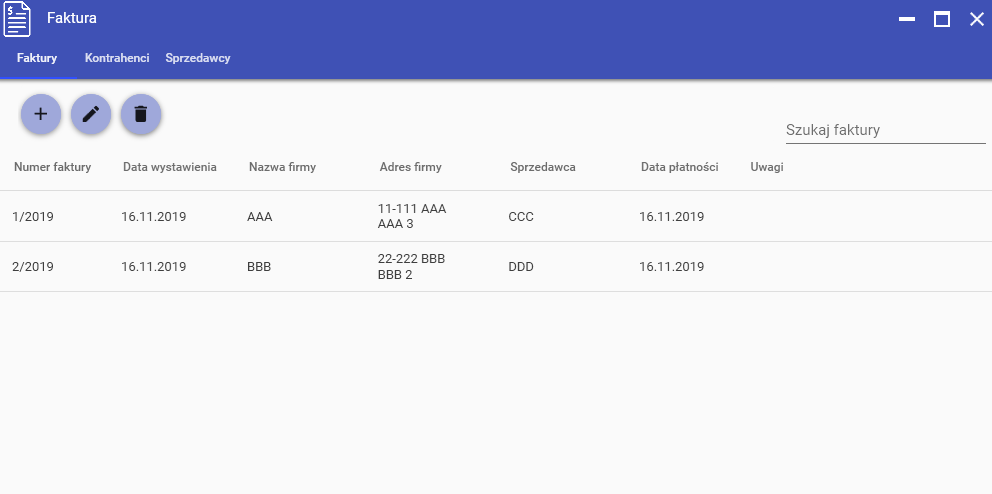
\includegraphics[width=\linewidth]{Rysunki/Main/InvoiceView.png}
  \caption{Okno widoku faktur}
  \label{fig:AddCustomerWindowInvoice}
\end{figure}

Aplikacja wyświetla nam wszystkie dostępne faktury \ref{fig:AddCustomerWindowInvoice}. Możemy zmienić widok na listę kontrahentów \ref{fig:AddCustomerWindowContractor} lub sprzedawców \ref{fig:AddCustomerWindowSeller}. 

\begin{figure}[ht!]
\centering
  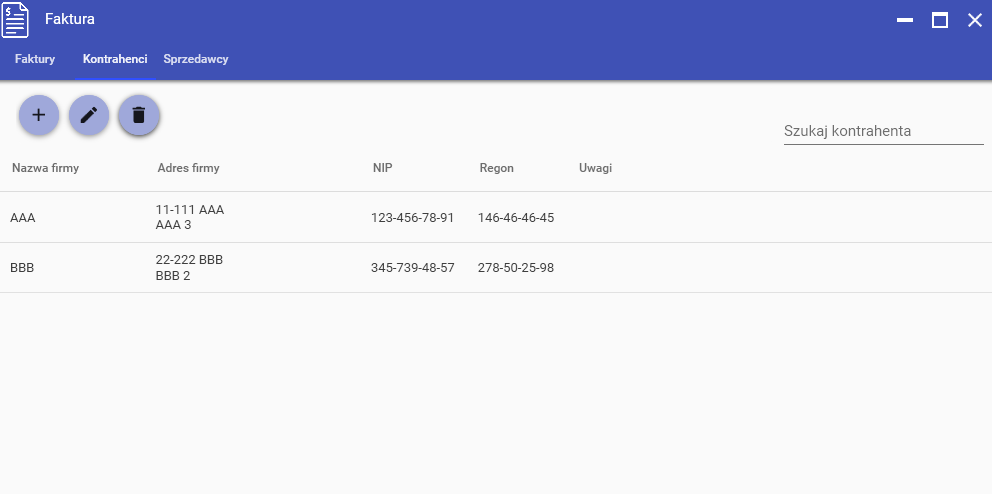
\includegraphics[width=\linewidth]{Rysunki/Main/contractorView.png}
  \caption{Okno widoku kontrahentów}
  \label{fig:AddCustomerWindowContractor}
\end{figure}

\begin{figure}[ht!]
\centering
  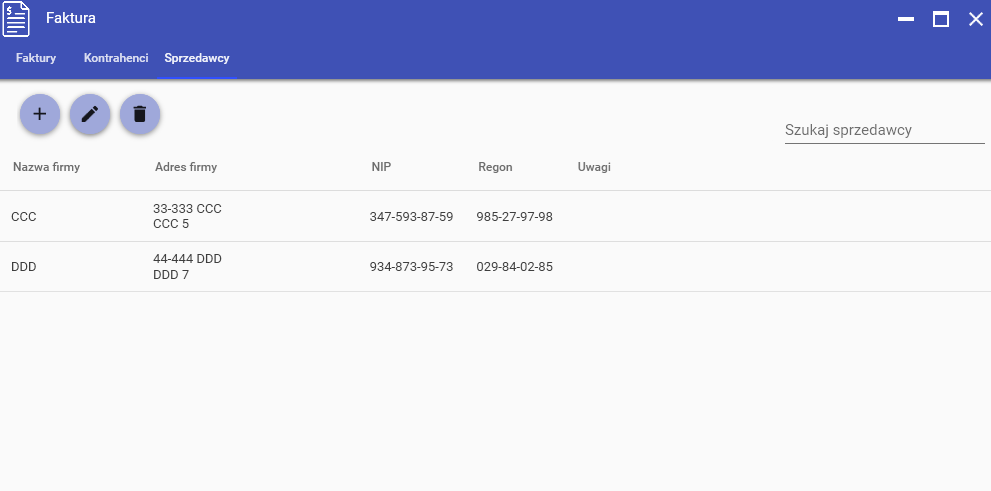
\includegraphics[width=\linewidth]{Rysunki/Main/sellerView.png}
  \caption{Okno widoku sprzedawców}
  \label{fig:AddCustomerWindowSeller}
\end{figure}

W każdym z tych trzech widoków możemy wykonać 3 takie same operacje - Dodanie, Edycja, Usunięcie. Każda z zakładek posiada również funkcjonalność szukania \ref{fig:AddCustomerWindowSearch}, która jest bardzo przydatna w przypadku dużej ilości pozycji na listach. Podczas usuwania faktury \ref{fig:AddCustomerWindowDeleteInvoice} użytkownikowi wyświetlany jest stosowny komunikat, który żąda potwierdzenia usunięcia faktury.

\begin{figure}[ht!]
\centering
  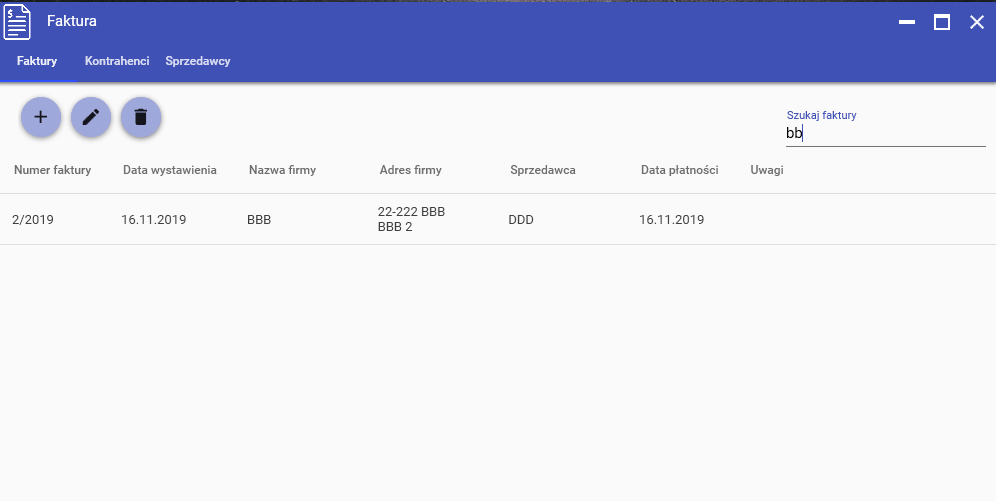
\includegraphics[width=\linewidth]{Rysunki/Main/MainSearch.png}
  \caption{Funkcja szukania}
  \label{fig:AddCustomerWindowSearch}
\end{figure}

\begin{figure}[ht!]
\centering
  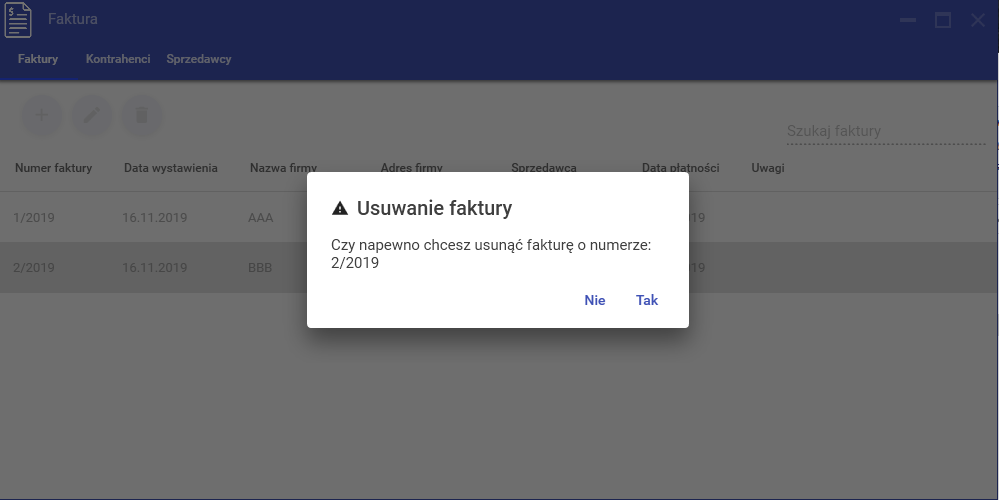
\includegraphics[width=\linewidth]{Rysunki/Main/deleteInvoiceView.png}
  \caption{Usuwanie faktury}
  \label{fig:AddCustomerWindowDeleteInvoice}
\end{figure}

\newpage~\newpage~\newpage~
\section{AddCustomerWindow}
Widok AddCustomerWindow jest oknem dodawania nowego kontrahenta lub sprzedawcy \ref{fig:AddCustomerWindow} (w zależności od tego jaki typ wybierzemy). 

\begin{figure}[ht!]
\centering
  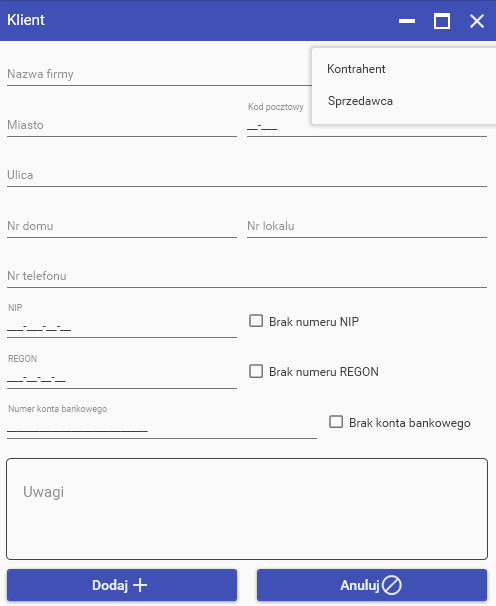
\includegraphics[width=0.7\linewidth]{Rysunki/AddCustomer/CustomerWindow.png}
  \caption{Okno widoku AddCustomerWindow}
  \label{fig:AddCustomerWindow}
\end{figure}

Wymaganymi wartościami do uzupełnienia są:

\begin{itemize}
    \item Nazwa firmy
    \item Miasto
    \item Ulica
    \item Numer domu
\end{itemize}

W przypadku, gdy nie podamy powyższych wartości nie będziemy w stanie zapisać nowego obiektu. Aplikacja wyświetli stosowny komunikat oraz zaznaczy pola, które zostały źle uzupełnione lub pominięte \ref{fig:AddCustomerWindowError}. 

\begin{figure}[ht!]
\centering
  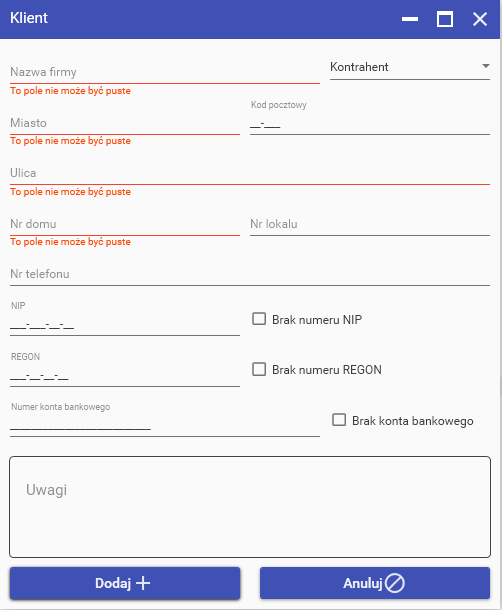
\includegraphics[width=0.7\linewidth]{Rysunki/AddCustomer/AddCustomerError.png}
  \caption{Widok pominiętych danych, które są wymagane}
  \label{fig:AddCustomerWindowError}
\end{figure}

\newpage~\newpage~
\section{InvoiceWindow}
Widok InvoiceWindow jest jednym z ważniejszych widoków w aplikacji. Na poniższym rysunku \ref{fig:InvoiceWindow} widoku możemy wybrać kontrahenta oraz sprzedawcę, na których będzie wypisana faktura. Następnie mamy możliwość wyboru daty wystawienia \ref{fig:InvoiceWindowDate} oraz zaznaczenia czy faktura będzie fakturą pro forma czy VAT. Poniżej wybieramy rodzaj płatności (gotówka, przelew lub płatność kartą), termin do kiedy faktura musi zostać opłacona oraz opcjonalnie (jeżeli została już opłacona) datę opłacenia faktury.

\begin{figure}[ht!]
\centering
  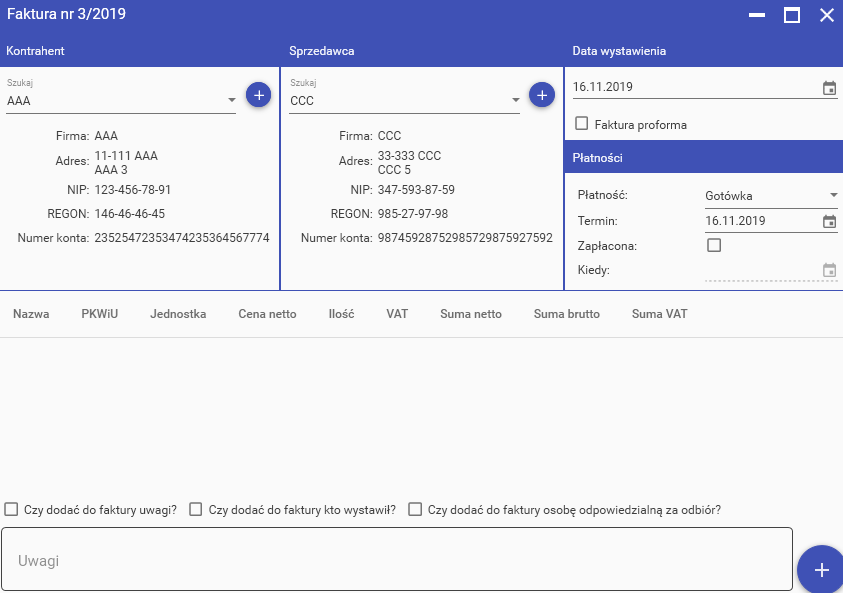
\includegraphics[width=\linewidth]{Rysunki/Invoice/InvoiceWindow.png}
  \caption{Okno widoku dodawania faktury}
  \label{fig:InvoiceWindow}
\end{figure}

\begin{figure}[ht!]
\centering
  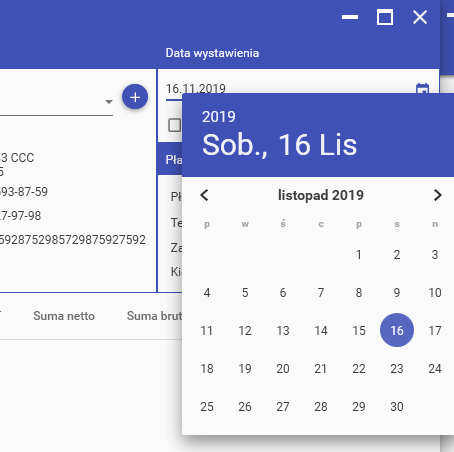
\includegraphics[width=0.5\linewidth]{Rysunki/Invoice/InvoiceSelectDate.png}
  \caption{Okno wyboru daty}
  \label{fig:InvoiceWindowDate}
\end{figure}

W prawym dolnym rogu znajduje się przycisk z ,,plusikiem'', który po kliknięciu otwiera nam menu opcji \ref{fig:InvoiceWindowMenu}. Pierwsze trzy przyciski służą do operacji na pozycjach znajdujących się na fakturze. Kolejne dwa pozwalają wygenerować fakturę VAT oraz jej korektę w przypadku jakichkolwiek zmian.

\begin{figure}[ht!]
\centering
  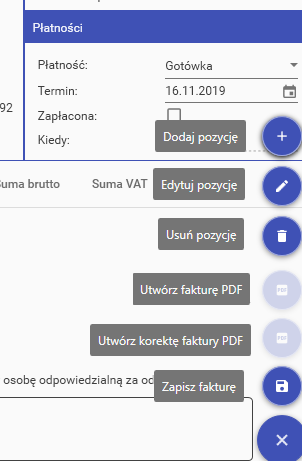
\includegraphics[width=0.5\linewidth]{Rysunki/Invoice/InvoiceMenu.png}
  \caption{Menu opcji na widoku InvoiceWindow}
  \label{fig:InvoiceWindowMenu}
\end{figure}

Rysunek \ref{fig:InvoiceWindowEdit} prezentuje nam fakturę w trybie podglądu. Na początku wszystkie kontrolki są wyłączone. W celu przejścia do trybu edycji użytkownik musi kliknąć przycisk ,,Edytuj fakturę''. W trybie podglądu aktywne są tylko 4 przyciski, które pozwalają na dodanie pól do pliku PDF z fakturą: 

\begin{itemize}
    \item Faktura proforma
    \item Czy dodać do faktury uwagi?
    \item Czy dodać do faktury kto wystawił?
    \item Czy dodać do faktury osobę odpowiedzialną za odbiór?
\end{itemize}

\begin{figure}[ht!]
\centering
  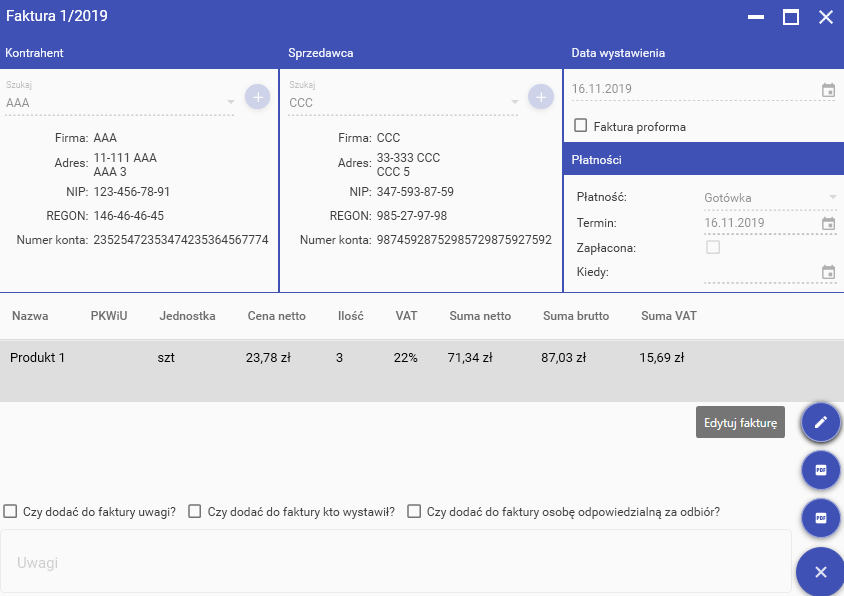
\includegraphics[width=\linewidth]{Rysunki/Invoice/InvoiceEdit.png}
  \caption{Okno widoku podglądu faktury}
  \label{fig:InvoiceWindowEdit}
\end{figure}

\newpage~\newpage~\newpage~
\section{InvoiceItemWindow}
Widok InvoiceItemWindow \ref{fig:InvoiceItemWindow} jest oknem dodawania pozycji do faktury.

\begin{figure}[ht!]
\centering
  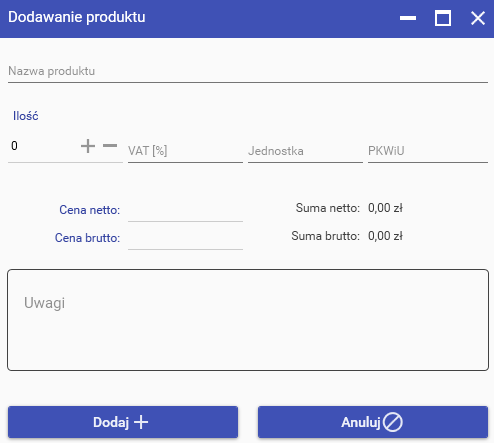
\includegraphics[width=\linewidth]{Rysunki/InvoiceItem/InvoiceItemWindow.png}
  \caption{Okno widoku dodawania pozycji do faktury}
  \label{fig:InvoiceItemWindow}
\end{figure}

Wymagane pola na widoku to InvoiceItemWindow to: 
\begin{itemize}
    \item Nazwa produktu
    \item VAT [\%]
    \item Jednostka
    \item Cenna netto lub brutto (jedna liczona na podstawie drugiej)
\end{itemize}

\newpage
W przypadku niepodania któregoś w powyższych pól, użytkownik otrzyma odpowiedni komunikat \ref{fig:InvoiceItemWindowError}.

\begin{figure}[ht!]
\centering
  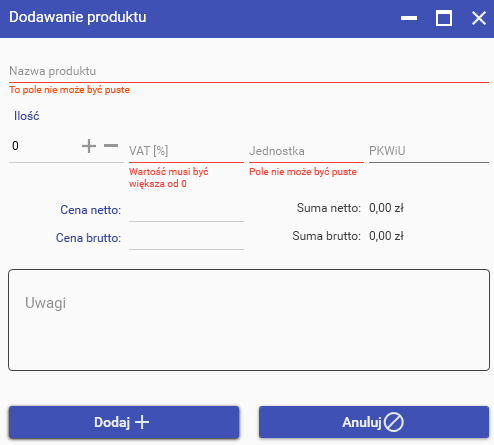
\includegraphics[width=\linewidth]{Rysunki/InvoiceItem/InvoiceItemWindowError.png}
  \caption{Błąd przy dodawaniu pozycji (niewypełnione pola)}
  \label{fig:InvoiceItemWindowError}
\end{figure}